% Options for packages loaded elsewhere
\PassOptionsToPackage{unicode}{hyperref}
\PassOptionsToPackage{hyphens}{url}
%
\documentclass[
]{book}
\usepackage{lmodern}
\usepackage{amssymb,amsmath}
\usepackage{ifxetex,ifluatex}
\ifnum 0\ifxetex 1\fi\ifluatex 1\fi=0 % if pdftex
  \usepackage[T1]{fontenc}
  \usepackage[utf8]{inputenc}
  \usepackage{textcomp} % provide euro and other symbols
\else % if luatex or xetex
  \usepackage{unicode-math}
  \defaultfontfeatures{Scale=MatchLowercase}
  \defaultfontfeatures[\rmfamily]{Ligatures=TeX,Scale=1}
\fi
% Use upquote if available, for straight quotes in verbatim environments
\IfFileExists{upquote.sty}{\usepackage{upquote}}{}
\IfFileExists{microtype.sty}{% use microtype if available
  \usepackage[]{microtype}
  \UseMicrotypeSet[protrusion]{basicmath} % disable protrusion for tt fonts
}{}
\makeatletter
\@ifundefined{KOMAClassName}{% if non-KOMA class
  \IfFileExists{parskip.sty}{%
    \usepackage{parskip}
  }{% else
    \setlength{\parindent}{0pt}
    \setlength{\parskip}{6pt plus 2pt minus 1pt}}
}{% if KOMA class
  \KOMAoptions{parskip=half}}
\makeatother
\usepackage{xcolor}
\IfFileExists{xurl.sty}{\usepackage{xurl}}{} % add URL line breaks if available
\IfFileExists{bookmark.sty}{\usepackage{bookmark}}{\usepackage{hyperref}}
\hypersetup{
  pdftitle={Datenanalyse mit R},
  pdfauthor={Marco},
  hidelinks,
  pdfcreator={LaTeX via pandoc}}
\urlstyle{same} % disable monospaced font for URLs
\usepackage{color}
\usepackage{fancyvrb}
\newcommand{\VerbBar}{|}
\newcommand{\VERB}{\Verb[commandchars=\\\{\}]}
\DefineVerbatimEnvironment{Highlighting}{Verbatim}{commandchars=\\\{\}}
% Add ',fontsize=\small' for more characters per line
\usepackage{framed}
\definecolor{shadecolor}{RGB}{248,248,248}
\newenvironment{Shaded}{\begin{snugshade}}{\end{snugshade}}
\newcommand{\AlertTok}[1]{\textcolor[rgb]{0.94,0.16,0.16}{#1}}
\newcommand{\AnnotationTok}[1]{\textcolor[rgb]{0.56,0.35,0.01}{\textbf{\textit{#1}}}}
\newcommand{\AttributeTok}[1]{\textcolor[rgb]{0.77,0.63,0.00}{#1}}
\newcommand{\BaseNTok}[1]{\textcolor[rgb]{0.00,0.00,0.81}{#1}}
\newcommand{\BuiltInTok}[1]{#1}
\newcommand{\CharTok}[1]{\textcolor[rgb]{0.31,0.60,0.02}{#1}}
\newcommand{\CommentTok}[1]{\textcolor[rgb]{0.56,0.35,0.01}{\textit{#1}}}
\newcommand{\CommentVarTok}[1]{\textcolor[rgb]{0.56,0.35,0.01}{\textbf{\textit{#1}}}}
\newcommand{\ConstantTok}[1]{\textcolor[rgb]{0.00,0.00,0.00}{#1}}
\newcommand{\ControlFlowTok}[1]{\textcolor[rgb]{0.13,0.29,0.53}{\textbf{#1}}}
\newcommand{\DataTypeTok}[1]{\textcolor[rgb]{0.13,0.29,0.53}{#1}}
\newcommand{\DecValTok}[1]{\textcolor[rgb]{0.00,0.00,0.81}{#1}}
\newcommand{\DocumentationTok}[1]{\textcolor[rgb]{0.56,0.35,0.01}{\textbf{\textit{#1}}}}
\newcommand{\ErrorTok}[1]{\textcolor[rgb]{0.64,0.00,0.00}{\textbf{#1}}}
\newcommand{\ExtensionTok}[1]{#1}
\newcommand{\FloatTok}[1]{\textcolor[rgb]{0.00,0.00,0.81}{#1}}
\newcommand{\FunctionTok}[1]{\textcolor[rgb]{0.00,0.00,0.00}{#1}}
\newcommand{\ImportTok}[1]{#1}
\newcommand{\InformationTok}[1]{\textcolor[rgb]{0.56,0.35,0.01}{\textbf{\textit{#1}}}}
\newcommand{\KeywordTok}[1]{\textcolor[rgb]{0.13,0.29,0.53}{\textbf{#1}}}
\newcommand{\NormalTok}[1]{#1}
\newcommand{\OperatorTok}[1]{\textcolor[rgb]{0.81,0.36,0.00}{\textbf{#1}}}
\newcommand{\OtherTok}[1]{\textcolor[rgb]{0.56,0.35,0.01}{#1}}
\newcommand{\PreprocessorTok}[1]{\textcolor[rgb]{0.56,0.35,0.01}{\textit{#1}}}
\newcommand{\RegionMarkerTok}[1]{#1}
\newcommand{\SpecialCharTok}[1]{\textcolor[rgb]{0.00,0.00,0.00}{#1}}
\newcommand{\SpecialStringTok}[1]{\textcolor[rgb]{0.31,0.60,0.02}{#1}}
\newcommand{\StringTok}[1]{\textcolor[rgb]{0.31,0.60,0.02}{#1}}
\newcommand{\VariableTok}[1]{\textcolor[rgb]{0.00,0.00,0.00}{#1}}
\newcommand{\VerbatimStringTok}[1]{\textcolor[rgb]{0.31,0.60,0.02}{#1}}
\newcommand{\WarningTok}[1]{\textcolor[rgb]{0.56,0.35,0.01}{\textbf{\textit{#1}}}}
\usepackage{longtable,booktabs}
% Correct order of tables after \paragraph or \subparagraph
\usepackage{etoolbox}
\makeatletter
\patchcmd\longtable{\par}{\if@noskipsec\mbox{}\fi\par}{}{}
\makeatother
% Allow footnotes in longtable head/foot
\IfFileExists{footnotehyper.sty}{\usepackage{footnotehyper}}{\usepackage{footnote}}
\makesavenoteenv{longtable}
\usepackage{graphicx,grffile}
\makeatletter
\def\maxwidth{\ifdim\Gin@nat@width>\linewidth\linewidth\else\Gin@nat@width\fi}
\def\maxheight{\ifdim\Gin@nat@height>\textheight\textheight\else\Gin@nat@height\fi}
\makeatother
% Scale images if necessary, so that they will not overflow the page
% margins by default, and it is still possible to overwrite the defaults
% using explicit options in \includegraphics[width, height, ...]{}
\setkeys{Gin}{width=\maxwidth,height=\maxheight,keepaspectratio}
% Set default figure placement to htbp
\makeatletter
\def\fps@figure{htbp}
\makeatother
\setlength{\emergencystretch}{3em} % prevent overfull lines
\providecommand{\tightlist}{%
  \setlength{\itemsep}{0pt}\setlength{\parskip}{0pt}}
\setcounter{secnumdepth}{5}
\usepackage{booktabs}
\usepackage[]{natbib}
\bibliographystyle{apalike}

\title{Datenanalyse mit R}
\author{Marco}
\date{2020-03-18}

\begin{document}
\maketitle

{
\setcounter{tocdepth}{1}
\tableofcontents
}
\hypertarget{preface}{%
\chapter*{Preface}\label{preface}}
\addcontentsline{toc}{chapter}{Preface}

{[}Work in Process{]}

\hypertarget{einleitung}{%
\chapter*{Einleitung}\label{einleitung}}
\addcontentsline{toc}{chapter}{Einleitung}

tbc\ldots{}

\hypertarget{who-will-find-this-book-useful}{%
\section*{Who will find this book useful?}\label{who-will-find-this-book-useful}}
\addcontentsline{toc}{section}{Who will find this book useful?}

Das Buch ist als Ergänzung zur Data-Übung gedacht\ldots{}

\hypertarget{getting-started}{%
\chapter{Getting started}\label{getting-started}}

tbc..

\hypertarget{kurzinfos-zur-entwicklung}{%
\section{Kurzinfos zur Entwicklung}\label{kurzinfos-zur-entwicklung}}

A brief history of Time tbc\ldots{}

\hypertarget{warum-r}{%
\section{Warum R?}\label{warum-r}}

Traditionell wird in den Sozialwissenschaften mit SPSS oder Stata als Statistik- und Analyse-Software gearbeitet. Warum hat sich dann R als defacto Programmiersprache zur Datenanalyse entwickelt? Einige Argumente sprechen für R:

\begin{itemize}
\tightlist
\item
  R ist freie Software und Open Source.
\item
  R läuft sowohl auf Windows als auch auf Mac Os und Linux.
\item
  R hat eine große und sehr aktive Community. Die Community stellt vielfältige Lern-Ressourcen zur Verfügung und hilft bei Problemen. Wir werden noch kennenlernen, wie wir von der Community profitieren können.
\item
  R wird aktiv weiterentwickelt. Besonders wichtig sind dabei sogenannte Packages, die nicht nur die Arbeit erleichtern, sondern auch die Anwendung neuer Methoden ermöglichen.
\end{itemize}

Aber R muss auch erlernt werden. Und Software verunsichert uns häufig, wenn sie nicht auf einem Drag-and-Drop Prinzip basiert, sondern durch Programmiercode ausgeführt wird.

\hypertarget{installation}{%
\section{Installation}\label{installation}}

Bevor wir starten, müssen wir R zunächst installieren. Auf der Website des Cran-Projekts („The Comprehensive R Archive Network``) können wir R downloaden und installieren. Wir beachten einfach die Hinweise (\emph{„install R for the first time``}) auf der Homepage via \href{https://cran.r-project.org/}{Cran}. Wenn wir R auf unserem Computer installiert haben, dann können wir mit einem Doppelklick das Programm öffnen und in der R Console starten.

\hypertarget{die-console}{%
\section{Die Console}\label{die-console}}

Die R Console erinnert etwas an Windows 98. Deshalb installieren wir auch später Rstudio, dass uns die Arbeit erleichtert und eher unserem Selbstbild als erfolgreiche Analysten entspricht. Aber erstmal gucken wir uns die Console an.

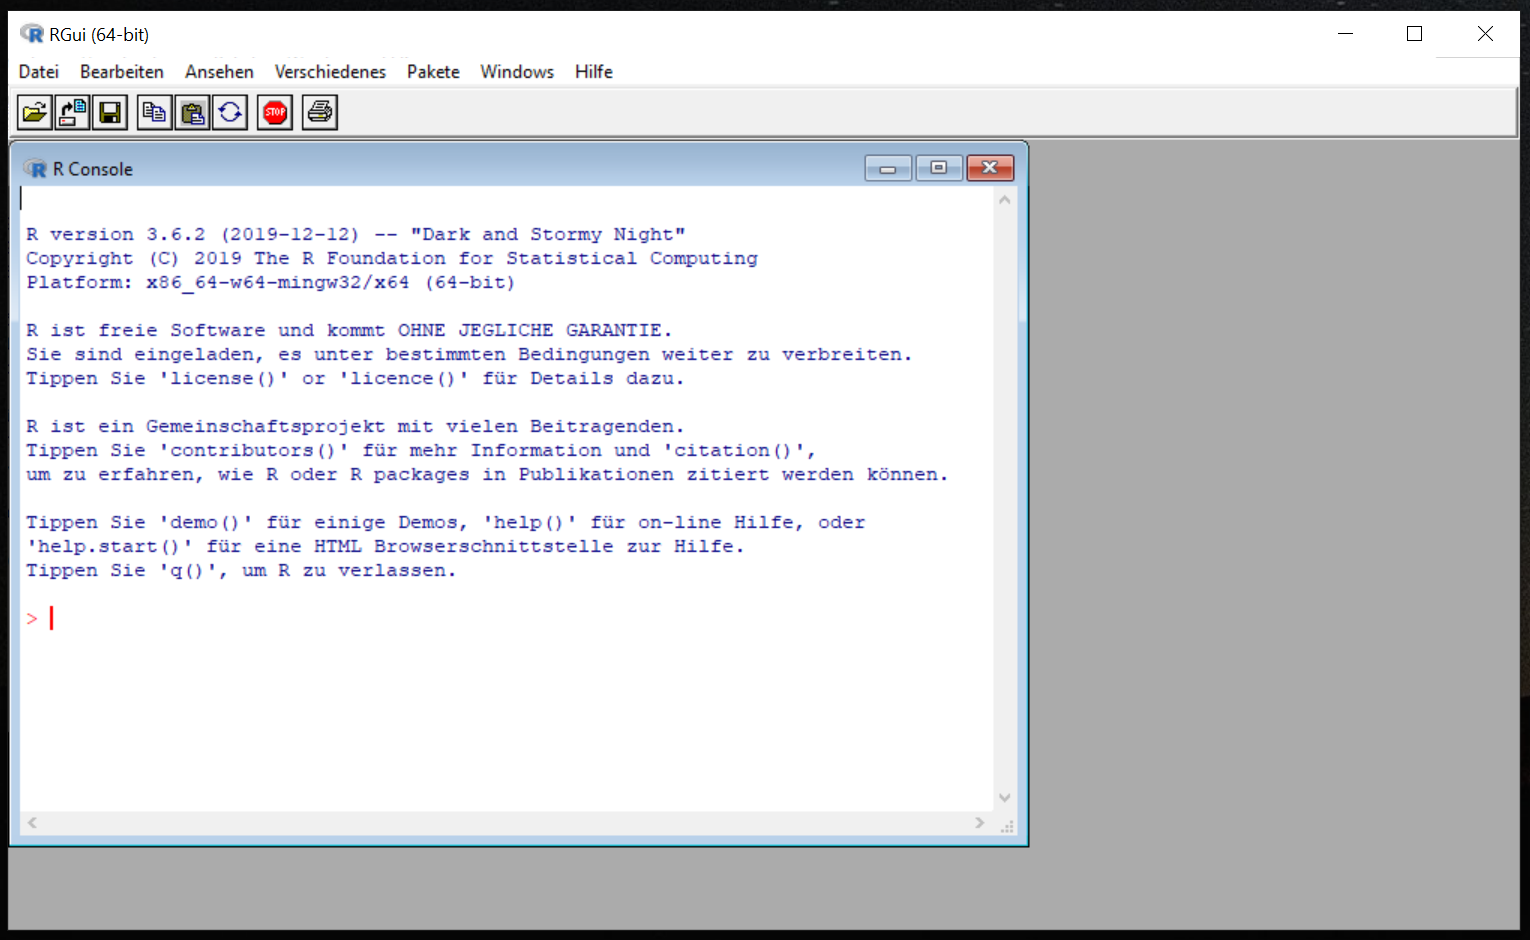
\includegraphics[width=21.25in]{img/s_r-console}
In der Console können wir direkt mit unserem Code beginnen. Um einen ersten Eindruck von R zu bekommen, halten wir uns an die alte Tradition ein Programm mit dem Ergebnis zu schreiben. Dafür nutzen wir die \texttt{print()} Funktion, geben in die Console \texttt{print(„Hello\ World!“)} ein und bestätigen mit Enter.

\begin{Shaded}
\begin{Highlighting}[]
\KeywordTok{print}\NormalTok{(}\StringTok{"Hello World!"}\NormalTok{)}
\CommentTok{## [1] "Hello World!"}
\end{Highlighting}
\end{Shaded}

Super, damit haben wir unseren ersten R Code geschrieben.
Die Console können wir aber auch als Taschenrechner nutzen: So können wir 15 Prozent Trinkgeld von unserem 35,70 Euro Bierdeckel in einer Kneipe berechnen, indem wir einfach 0.15 * 35.70 in die Console eingeben und mit Enter bestätigen.

\begin{Shaded}
\begin{Highlighting}[]
\FloatTok{0.15} \OperatorTok{*}\StringTok{ }\FloatTok{35.70}
\CommentTok{## [1] 5.355}
\end{Highlighting}
\end{Shaded}

Das Ergebnis lautet 5,35 Euro. Falls ein Fehler auftritt, könnte dies an einem Komma \texttt{,} anstatt einem Punkt \texttt{.} zur Trennung liegen.

\hypertarget{rstudio}{%
\section{RStudio}\label{rstudio}}

\hypertarget{pakate}{%
\section{Pakate}\label{pakate}}

\hypertarget{styleguide}{%
\chapter{Styleguide}\label{styleguide}}

\hypertarget{gute-praxis}{%
\section{Gute Praxis}\label{gute-praxis}}

wie schreibe ich ``guten'' Code

\hypertarget{r-projekte}{%
\section{R Projekte}\label{r-projekte}}

Ziel: Ein R Projekt und entsprechende Unterordner anlegen, um nicht die Übersicht zu verlieren. Kurzer Abschnitt, wie Pfade definiert und gesetzt werden.
Organisation eines Projekts

\begin{itemize}
\tightlist
\item
  R Projekt

  \begin{itemize}
  \tightlist
  \item
    set-up.R
  \item
    R Code
  \item
    Input
  \item
    Grafiken
  \item
    Output
  \end{itemize}
\end{itemize}

\hypertarget{trial-and-error}{%
\section{Trial and Error}\label{trial-and-error}}

\hypertarget{help}{%
\section{Help}\label{help}}

tbc

  \bibliography{book.bib}

\end{document}
